\documentclass[12pt]{article}

\usepackage{url,graphicx,amssymb,lastpage}

\usepackage[usenames,dvipsnames,table]{xcolor}

\usepackage{listings}
\definecolor{codegreen}{rgb}{0,0.6,0}
\definecolor{codegray}{rgb}{0.5,0.5,0.5}
\definecolor{codepurple}{rgb}{0.58,0,0.82}
\definecolor{backcolour}{rgb}{0.9,0.9,0.9}
\lstdefinestyle{mystyle}{
    backgroundcolor=\color{backcolour},   
    commentstyle=\color{codegreen},
    keywordstyle=\color{magenta},
    numberstyle=\tiny\color{codegray},
    stringstyle=\color{codepurple},
    basicstyle=\footnotesize\tt,
    breakatwhitespace=false,
    breaklines=true,
    captionpos=b,
    keepspaces=true,
%     numbers=false,
    numbersep=5pt,
    showspaces=false,
    showstringspaces=false,
    showtabs=false,
    tabsize=2
}
 
\lstset{style=mystyle}
 


\usepackage{soul}
\setuldepth{a}

\usepackage{cmbright}
\usepackage[T1]{fontenc}

\usepackage[normalem]{ulem}

\usepackage{fancyhdr}

\pagestyle{fancy}
\renewcommand{\headrulewidth}{0pt}
% \fancyhead[LEO]{\textcolor[gray]{0.4}{Neil Vaytet \hfill \acronym -- Standard EF}}
\fancyhead[CEO]{\textcolor[gray]{0.4}{Plotting-Ramses User Guide}}
% \fancyfoot[LEO]{\textcolor[gray]{0.4}{H2020-MSCA-IF-2014-Standard EF \hfill Part B -- Page \thepage ~of \pageref*{LastPage}}}
\fancyfoot[CEO]{\textcolor[gray]{0.4}{Page \thepage ~of \pageref*{LastPage}}}
% \fancyfoot[LEO]{\textcolor[gray]{0.4}{Neil Vaytet \hfill Part B -- Page \thepage ~of \pageref*{LastPage}}}

% \cfoot{}
\rhead{}
\lhead{}
% \renewcommand{\contentsname}{\hfill TABLE OF CONTENTS \hfill}

\usepackage[pdftex]{hyperref}
\hypersetup{colorlinks=true,linkcolor=black,citecolor=blue,urlcolor=blue}
\urlstyle{sf}

\topmargin -0.40in
\textheight 9.0in
\oddsidemargin 0.0in
\evensidemargin 0.0in
\textwidth 6.5in
% \headsep 12pt
% \footskip 18pt

\setlength\headwidth{\textwidth}

%%%%%%%%%%%%%%%%%%%%%%%%%%%%%%%%%%%%%%%%%%%%%%%%%%%%%%%%%%%%%%%%%%%%%%%%%%%%%%%%%%%%%%%%%%%%%%%%%%%%%
%%%%%%%%%%%%%%%%%%%%%%%%%%%%%%%%%%%%%%%%%%%%%%%%%%%%%%%%%%%%%%%%%%%%%%%%%%%%%%%%%%%%%%%%%%%%%%%%%%%%%
%%%%%%%%%%%%%%%%%%%%%%%%%%%%%%%%%%%%%%%%%%%%%%%%%%%%%%%%%%%%%%%%%%%%%%%%%%%%%%%%%%%%%%%%%%%%%%%%%%%%%

\begin{document}

\begin{center}
\huge

\vspace*{50pt}

\textbf{Plotting-Ramses\\User Guide}

\thispagestyle{empty}

\vspace{50pt}

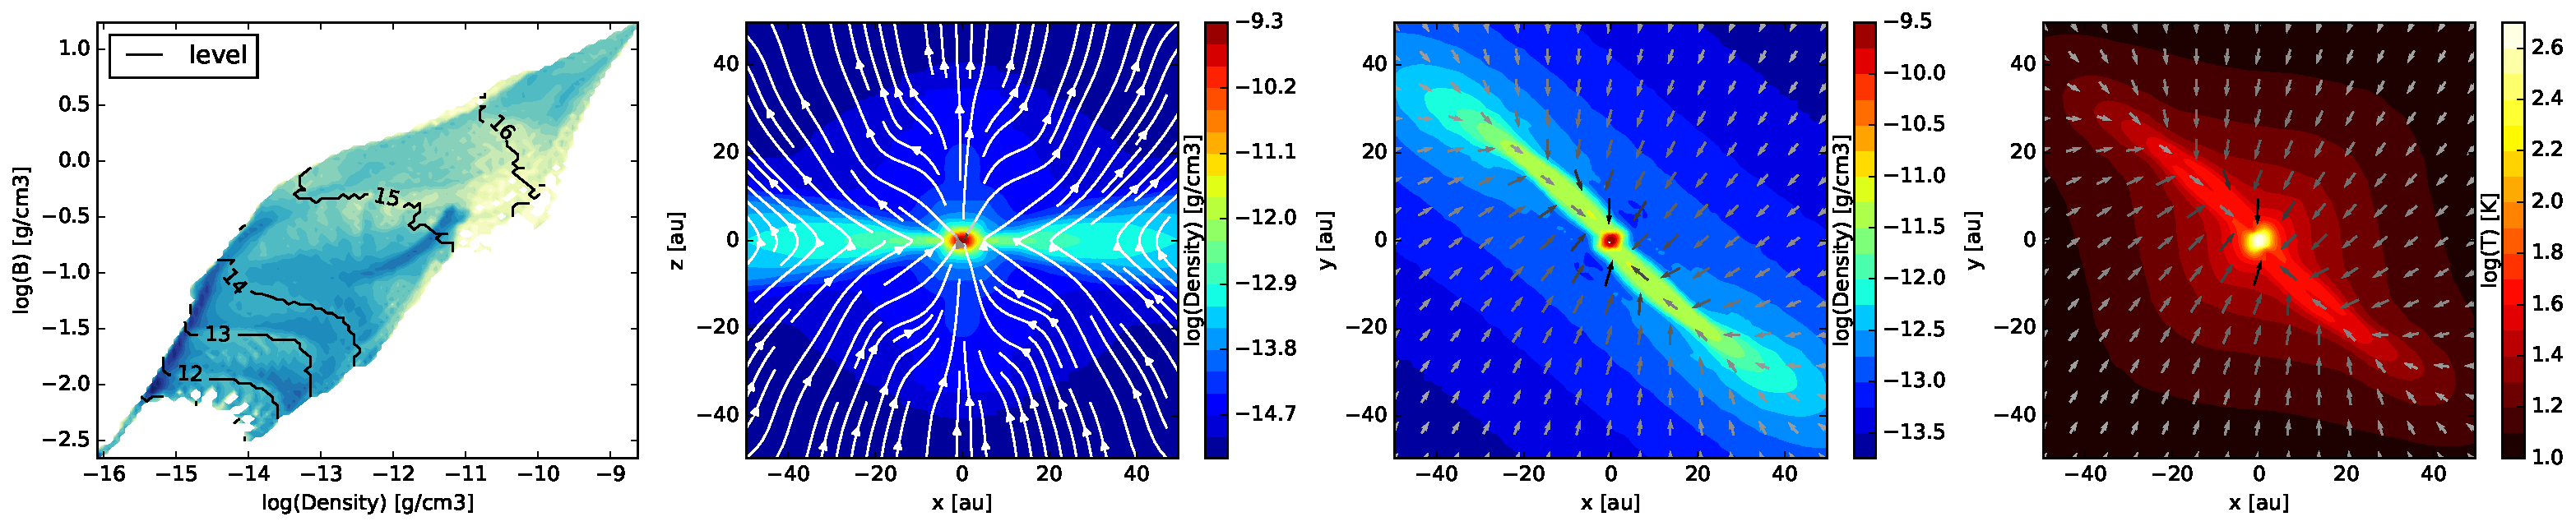
\includegraphics[width=\textwidth]{demo.pdf}

\Large

\vspace{100pt}

Neil Vaytet

\vspace{5pt}

Centre for Star and Planet Formation\\
Niels Bohr Institute\\
University of Copenhagen\\
Denmark

\vspace{5pt}

\textcolor{blue}{\texttt{neil.vaytet@nbi.ku.dk}}

\vspace{70pt}

Version 1.0 - 18/03/2017

\end{center}

\clearpage

\tableofcontents

\clearpage



\section{Introduction}

Plotting-Ramses was developed to provide a light-weight method to read and plot basic diagnostics on \href{https://bitbucket.org/rteyssie/ramses}{\texttt{RAMSES}} simulation outputs. It currently only works with the native `binary' data output format. It uses \texttt{f2py} to interface a fast \texttt{Fortran90} file reader with a \texttt{Python-matplotlib} layer for data manipulation and visualization.

\section{Getting started}

\subsection{Installation}

\textbf{Requirements}: you will need matplotlib and \texttt{f2py} installed on your system.\\
Clone the repository from \href{https://bitbucket.org/nvaytet/plotting-ramses}{\texttt{Bitbucket}} into your chosen directory. For this tutorial, the directory will be located at \texttt{/home/user/software}:
\begin{lstlisting}
cd /home/user/software
git clone https://nvaytet@bitbucket.org/nvaytet/plotting-ramses.git
\end{lstlisting}
Before plotting, you must first run '\texttt{f2py}' on the fortran subroutine which reads in the \texttt{RAMSES} data:
\begin{lstlisting}
cd plotting-ramses
f2py -c read_ramses_data.f90 -m read_ramses_data
\end{lstlisting}
This will print out a few warnings but should still create a file \texttt{read\_ramses\_data.so} in the \texttt{plotting-ramses} directory.
Finally, it would probably be a good idea to add the path to the \texttt{plotting-ramses} directory to you \texttt{PYTHONPATH}:
\begin{lstlisting}
export PYTHONPATH=$PYTHONPATH:/home/user/software/plotting-ramses
\end{lstlisting}
To avoid having to do this every time you open a new terminal, you can of course add this to you \texttt{.bashrc} file.

\subsection{Making your first plot}

Navigate to the directory containing the data of your simulation and open an \texttt{ipython} console:
\begin{lstlisting}
cd /path/to/my/ramses/data
ipython
\end{lstlisting}
Import the \texttt{plotting\_ramses} class and load the output of your choice (this will be output number 71 in this example).\footnote{The data loader searches for a \texttt{hydro\_file\_descriptor.txt} inside the output directory to get the variable names, so make sure your version of \texttt{RAMSES} supports this. If it doesn't, you can edit the \texttt{read\_ramses\_data.f90} subroutine so that it reads the data properly. By default it will try to guess by itself which are the variables to read, but this will almost certainly fail with editing it.}
\begin{lstlisting}
In [1]: import plotting_ramses as pp
In [2]: mydata = pp.RamsesOutput(71,scale="au",verbose=True)
============================================
Processing    60 files
 10%
 20%
 30%
 40%
 50%
 60%
 70%
 80%
 90%
100%
Read   2458296 cells
Generating data structure... please wait
output_00071 successfully loaded
--------------------------------------------
boxsize: 11034.1000058
center: None
levelmax: 29
levelmin: 6
ncells: 2458296
ncpu: 60
ndim: 3
nstep: 700
scale: au
time: 8.990163083e+11
ud: 3.8346e-24
ul: 3.08e+18
ut: 1.97732040947e+15
--------------------------------------------
The variables are:
Name               Unit      Min               Max          
B                  [G      ] 7.05568663006e-06 18.1223463688    
B_left_x           [G      ] -4.30285430461    4.30285430335    
B_left_y           [G      ] -5.24127101488    5.24127101996    
B_left_z           [G      ] -0.202153242353   18.1962401627    
B_right_x          [G      ] -4.30285430461    4.30285430335    
B_right_y          [G      ] -5.24127101488    5.24127101996    
B_right_z          [G      ] -0.202153242353   18.1962401627    
B_x                [G      ] -4.29553104763    4.29553104622    
B_y                [G      ] -5.18964286611    5.18964287075    
B_z                [G      ] -0.200583478476   18.1221774265    
density            [g/cm3  ] 1.53759058663e-20 2.62851267815e-09
dx                 [au     ] 0.0841835022417   172.407812591    
level              [       ] 6.0               17.0             
log_B              [g/cm3  ] -5.15146071612    1.25821442673    
log_T              [K      ] 0.977980673125    2.84825249049    
log_rho            [g/cm3  ] -19.8131592885    -8.5802899239    
passive_scalar_1   [       ] 0.0               0.0              
passive_scalar_2   [       ] 0.0               0.0              
passive_scalar_3   [       ] 0.0               0.0              
passive_scalar_4   [       ] 209.455501728     24103.1825934    
radiative_energy_1 [erg/cm3] 6.24769168451e-11 0.0018699559894  
temperature        [K      ] 9.50562490999     705.102883133    
thermal_pressure   [g/cm/s2] 5.23633293194e-12 102.480387715    
velocity_x         [cm/s   ] -267066.601808    267066.601866    
velocity_y         [cm/s   ] -258785.071957    258785.071989    
velocity_z         [cm/s   ] -174910.102931    174904.922142    
x                  [au     ] -5430.84609661    5430.84609661    
y                  [au     ] -5430.84609661    5430.84609661    
z                  [au     ] -5430.84609661    5430.84609661    
============================================
\end{lstlisting}
In the call to \texttt{RamsesOutput}, the first argument is the output number\footnote{Note that you can use "\texttt{-1}" to select the last output in the directory.}, while the second is the spatial scale you want to convert distances to. Possible choices are "\texttt{cm}", "\texttt{au}" or "\texttt{pc}".
If you add \texttt{`verbose=True'} to the argument list, it will also print out some information about the data (the variables names, their minimum and maximum values, etc.). \texttt{plotting-ramses} tries to guess the units of each variable field according to its name. This is done by the \texttt{get\_units()} function and can easily be modified if you have non-standard variables.\\
\\
We now wish to plot a 2d histogram of the logarithm of density versus logarithm of magnetic field for all the cells inside the computational domain.
\begin{lstlisting}
In [3]: mydata.plot_histogram("log_rho","log_B")
\end{lstlisting}

\section{Support}

Plotting-Ramses was developed by Neil Vaytet \& Tommaso Grassi from the Centre for Star and Planet Formation at the University of Copenhagen, Denmark.

\noindent The software is free for anyone to use, but absolutely no warranty is provided. If you run into bugs or issues, you can contact the authors via email at \textcolor{blue}{\texttt{neil.vaytet@nbi.ku.dk}}.

\end{document}

